% question 6

\section{Question 6}

\paragraph{(a)} The dynamic equation of mechanical system formed by a mass block, spring and damper is given by
\begin{equation}
	M \ddot{x}_m = F_m - B_m \dot{x}_m - F_l,
	\label{eq:q6_dyn}
\end{equation}
\noindent where $M$ is system mass, $x_m$ is block position, $F_m$ control force, $B_m$ is damping constant and $F_l$ is force generated by spring. Then, \eqref{eq:q6_dyn} can be represented in Laplace space as
\begin{equation}
	(M s^2 + B_m s)X_m (s) = F_m(s) - F_l(s).
	 \label{eq:q6_dyn_laplace}
\end{equation}

The force generated by spring can be computed as $F_l = k (x_m - x_l)$, where $k$ is spring constant and $x_l$ is load position. Hence, considering $X_m(s)=\frac{F_l(s)}{k} + X_l(s)$, \eqref{eq:q6_dyn_laplace} can be described in terms of $F_m(s)$, $F_l(s)$ and $X_l(s) $
\begin{equation}
	F_l(s) = \frac{k}{M s^2 + B_m s + k} F_m(s) - \frac{Mks^2 + B_m k s}{M s^2 + B_m s + k} X_l(s).
\end{equation} 

Finally, $G_1(s)=\frac{k}{M s^2 + B_m s + k}$ and $G_2(s)= - \frac{Mks^2 + B_m k s}{M s^2 + B_m s + k}$.

\paragraph{(b)} Figure \ref{fig:q6_block_diagrama} describes the block diagram for force control of  mechanical system $\frac{F_l(s)}{F_m(s)} = \frac{k}{M s^2 + B_m s + k}$.

\begin{figure}[h!]
	\centering
	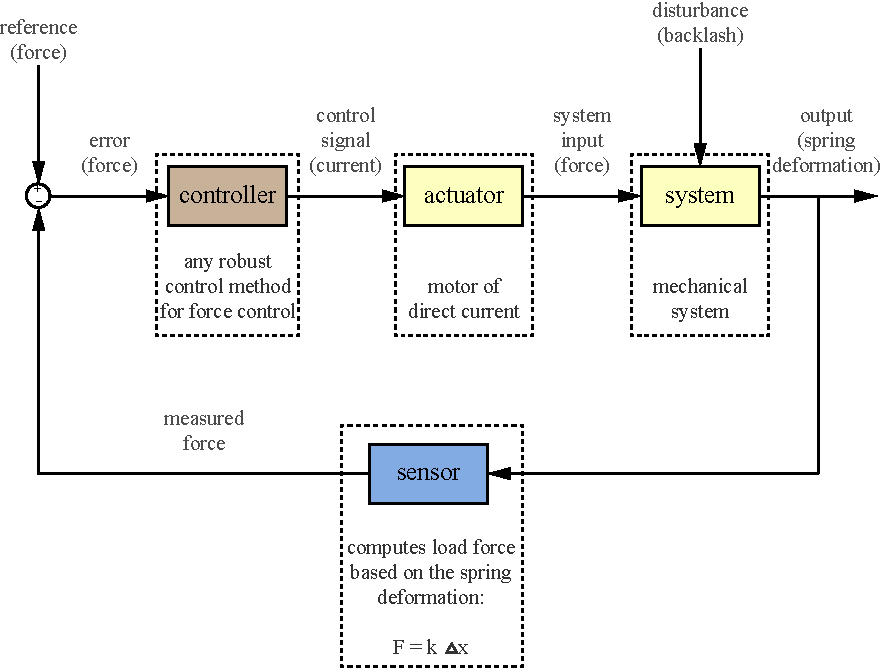
\includegraphics{q6.pdf}
	\caption{Block diagram for force control.}
	\label{fig:q6_block_diagrama}
\end{figure}

\paragraph{(c)} Figure \ref{fig:q6_step_response_G1} describes step response of open-loop system ( $G_1(s)=\frac{k}{M s^2 + B_m s + k}$).


\begin{figure}[h!]
	\centering
	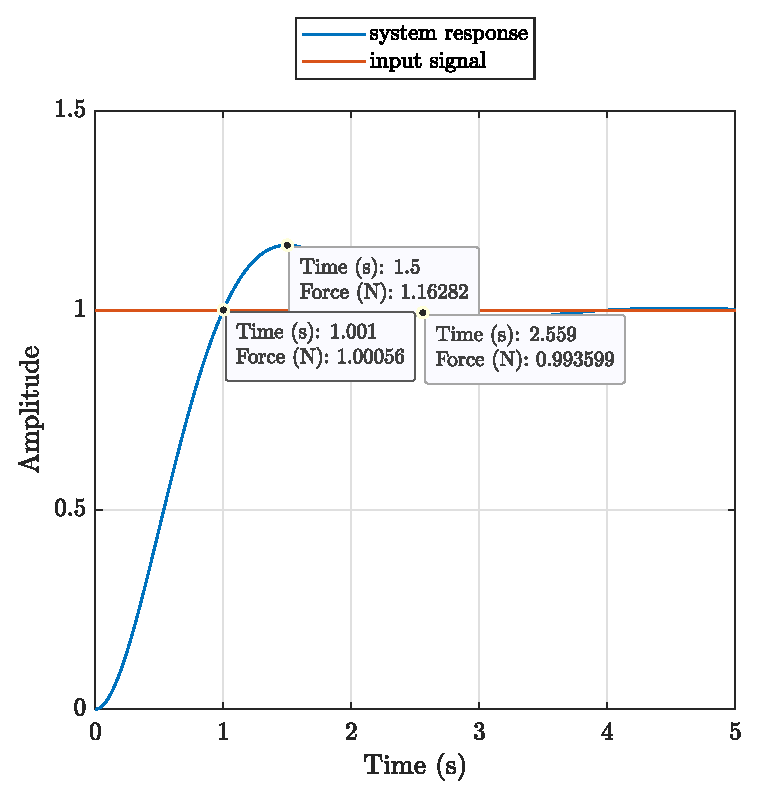
\includegraphics{q6_step_response_G1.eps}
	\caption{Step response of open-loop system ( $G_1(s)=\frac{k}{M s^2 + B_m s + k}$).}
	\label{fig:q6_step_response_G1}
\end{figure}

\paragraph{(d)} The step response indicates that overshoot is $\%PO \approx 35\%$, peak time is $t_p \approx 1.05$ s, rise time is $t_r \approx 0.63$ s and settling time is $t_s \approx 2.55$ s. The theoretical values indicates that overshoot is $\%PO = 35.09\%$, peak time is $t_p \approx 1.0472$ s, rise time is $t_r \approx 0.6308$ s and settling time is $t_s \approx 3$ s. Hence, values obtained from step response are close to theoretical ones.

\paragraph{(e)} In order to avoid damage human operator, is better have a slow response with overshoot close to $\% 0$ than a fast with high forces. Hence, close-loop system should be over-damping or critically damped, in this way, $\%PO \approx 0$ and  $t_s \approx 1.5$ second. 
